\documentclass[dvipdfmx,autodetect-engine]{beamer}

% 好みのテーマ(必要なら後で変更)
\usetheme{Madrid}
\usecolortheme{default}

% 共通前置き&マクロ
% ==== beamer 用(upLaTeX + dvipdfmx 前提)====

% 数式
\usepackage{amsmath,amssymb,mathtools,bm}
\allowdisplaybreaks

% 図(beamerはgraphicxを内部導入するが,dvipdfmx用途で明示してもよい)
\usepackage[dvipdfmx]{graphicx}

% ハイパーリンク:beamerがhyperrefを読むので,細部設定のみ
\hypersetup{
  hidelinks,
  pdfpagemode=UseNone,
  bookmarksnumbered=true
}

% ---- 文献(biblatex + biber 前提;Paperpileの .bib を主ファイル基準で)----
\usepackage{csquotes}
\usepackage[
  backend=biber,
  style=apa,      % 必要に応じて phys/authoryear へ差替え
  natbib=true
]{biblatex}
\addbibresource{paperpile.bib}

% 参照(定理名や図表名のスマート参照)
\usepackage[nameinlink,capitalise]{cleveref}

% 表(論文向けの見栄え)
\usepackage{booktabs,threeparttable,threeparttablex}
\usepackage{tabularx,array}
\renewcommand{\arraystretch}{1.1}

% 色
\usepackage{xcolor}

% 日本語(upLaTeX)
\usepackage[deluxe]{otf}
\usepackage[noalphabet]{pxchfon}
\renewcommand{\kanjifamilydefault}{\gtdefault}
\IfFileExists{HaranoAjiGothic-Medium.otf}{%
  \setboldgothicfont{HaranoAjiGothic-Medium.otf}%
}{}

% 図の相対パス
\graphicspath{{./figures/}}




% ==== メタ情報(必要に応じて毎回ここだけ更新)====
\newcommand{\papertitle}{N}
\newcommand{\paperauthor}{Koshi Harashima}
\newcommand{\paperaffil}{Northwestern University}
\newcommand{\paperdate}{October 6, 2025}

% ==== 数式系のマクロ ====
\newcommand*{\N}{\mathbb{N}}
\newcommand*{\Z}{\mathbb{Z}}
\newcommand*{\Q}{\mathbb{Q}}
\newcommand*{\R}{\mathbb{R}}
\newcommand*{\C}{\mathbb{C}}
\newcommand*{\I}{\mathbb{I}}

\newcommand*{\boldalpha}  {\boldsymbol \alpha}
\newcommand*{\boldbeta}   {\boldsymbol \beta}
\newcommand*{\boldgamma}  {\boldsymbol \gamma}
\newcommand*{\bolddelta}  {\boldsymbol \delta}
\newcommand*{\boldepsilon}{\boldsymbol \epsilon}
\newcommand*{\boldtheta}  {\boldsymbol \theta}

\DeclareMathOperator*{\esssup}{ess\,sup}

\usepackage{booktabs}

\title{\papertitle}
\author{\paperauthor}
\institute{\paperaffil}
\date{\paperdate}

\begin{document}

\AtBeginSection[]{
  \begin{frame}{目次(現在のセクション)}
    % currentsection オプションで,今のセクションだけを強調
    \tableofcontents[
      currentsection,        % 今のセクションを強調
      hideothersubsections   % ほかのセクションのサブセクションは隠す
    ]
  \end{frame}
}

\frame{\titlepage}

\begin{frame}{発表の概要}
  \begin{itemize}
    \item \textbf{3.6 層出力の正規化}
      \begin{itemize}
        \item 入力の標準化(平均0・分散1に移動)
        \item バッチ正規化(Batch Normalization)
        \item レイヤー正規化(Layer Normalization)
        \item 重み正規化と正則化
      \end{itemize}
    \item \textbf{3.7 重みの初期化}
      \begin{itemize}
        \item Xavier(Glorot)初期化
        \item Kaiming(He)初期化
      \end{itemize}
    \item \textbf{3.8 その他}
      \begin{itemize}
        \item カリキュラム学習(Curriculum Learning)
        \item 非凸損失関数と鞍点対策
      \end{itemize}
  \end{itemize}
\end{frame}

\section{3.6}
% Slide 1
\begin{frame}{3.6.1 概要}
\small
  \begin{itemize}
    \item 順伝播型ネットワークでは,入力が統計分布に従うと,\\
      各層出力も何らかの統計分布に従う
    \item 学習の途中で下位層の重みに応じた出力分布の変化が起きると,\\
      各層出力の分布が大きく変化し学習が不安定化する
    \item これを防ぐため,各層の出力を強制的に正規化(normalization)し,\\
      分布の形を整える手法を導入する
    \item 以降,まず入力の正規化(3.6.2),次に層出力の正規化(3.6.3~)を説明
  \end{itemize}
  \begin{figure}
      \centering
      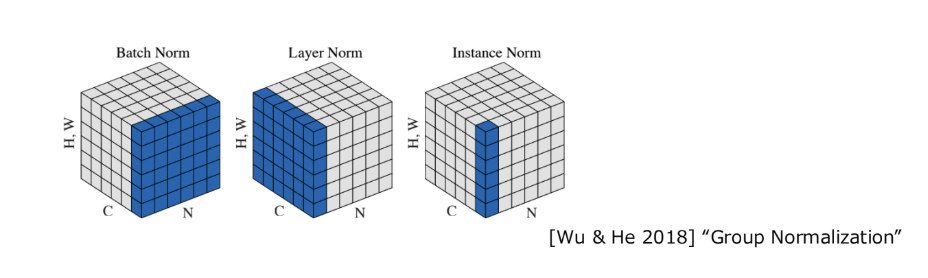
\includegraphics[width=0.8\textwidth]{Standalization.png}
    \caption*{Normalizationの方法集}
  \end{figure}
\end{frame}

\begin{frame}{正規化の背景}
  \begin{block}{共変量シフト (Covariate Shift)}
    \begin{itemize}
      \item 訓練時と推論時で入力データの分布が変化すると,  
            モデルの精度が大きく低下する
      \item 例:通常の MNIST で訓練 → 15° 回転 MNIST でテスト  
    \end{itemize}
  \end{block}
  \begin{block}{内部共変量シフト (Internal Covariate Shift)}
    \begin{itemize}
      \item ネットワーク内部の活性化分布が変わり続け,  
            各層の学習が非定常になる問題
      \item 解決策:各層の出力を毎回「平均0・分散1」の分布に正規化  
    \end{itemize}
  \end{block}
\end{frame}



% Slide 2
\begin{frame}{3.6.2 入力の正規化 (1)前処理の目的}
  \begin{block}{データ正規化(normalization)/標準化(standardization)}
    訓練データ 
    $\mathcal{D} = \{(x_n,y_n)\}_{n=1}^N$ 
    の各入力 $x_n$ に対し,
    \[
      x_{n,i} \leftarrow x_{n,i} - \bar{x}_i
      ,\quad
      \bar{x}_i = \frac{1}{N}\sum_{n=1}^N x_{n,i}
    \]
    を行い,変換後の平均を 0 にする.
  \end{block}
  \begin{itemize}
    \item 各成分ごとに平均0にすることで,分布の中心化を実現
    \item 続いて分散1へのスケーリングも行う
  \end{itemize}
\end{frame}

% Slide 3
\begin{frame}{3.6.2 入力の正規化 (2)分散でスケール調整}
  \begin{block}{標準化の式}
    \[
      \sigma_i 
      = \sqrt{\frac{1}{N}\sum_{n=1}^N (x_{n,i}-\bar{x}_i)^2}
      ,\quad
      x_{n,i} \leftarrow \frac{x_{n,i}-\bar{x}_i}{\sqrt{\sigma_i^2 + \varepsilon}}
    \]
    \begin{itemize}
      \item $\sigma_i$: 成分 $i$ の標本標準偏差
      \item $\varepsilon$: 分母ゼロ回避のための微小定数
    \end{itemize}
  \end{block}
  \begin{itemize}
    \item この2段階で訓練データの各成分は「平均0・分散1」となる
    \item 推論時には,訓練時に計算した $\bar{x}_i,\sigma_i$ を用いる
  \end{itemize}
  \begin{figure}
    \centering
    \includegraphics[width=0.4\textwidth]{図3_7.png}
    \caption*{図3.7(c) 分散1化}
  \end{figure}
\end{frame}

% Slide 4: Batch Normalization
\begin{frame}{3.6.3 バッチ正規化 (Batch Normalization)}
  \begin{itemize}
    \item ミニバッチ内の全サンプルに対して,各ユニットの平均・分散を計算
      \[
        \mu_j = \frac{1}{m}\sum_{n=1}^m u_j^{(n)},\quad
        \sigma_j^2 = \frac{1}{m}\sum_{n=1}^m (u_j^{(n)} - \mu_j)^2
      \]
    \item 正規化とアフィン変換
      \[
        \hat u_j^{(n)}
         = \frac{u_j^{(n)} - \mu_j}{\sqrt{\sigma_j^2 + \varepsilon}},\quad
        y_j^{(n)} = \gamma_j\,\hat u_j^{(n)} + \beta_j
      \tag{3.16}
      \]
    \item $\gamma_j, \beta_j$ は学習可能パラメータ(初期値 $\gamma_j=1,\ \beta_j=0$)
    \item 推論時は訓練中に移動平均で記録した $\mu_j,\sigma_j^2$ を使用
  \end{itemize}
\end{frame}

\begin{frame}{バッチ正規化 (Batch Normalization)}
  \[
    \mu_j = \frac1m\sum_{i=1}^m h_{i,j}, \quad
    \sigma_j^2 = \frac1m\sum_{i=1}^m (h_{i,j}-\mu_j)^2
  \]
  \[
    \hat h_{i,j}
      = \frac{h_{i,j}-\mu_j}{\sqrt{\sigma_j^2+\varepsilon}}, \quad
    y_{i,j}
      = \gamma_j\,\hat h_{i,j} + \beta_j
  \]
  \vspace{0.8em}
  \begin{figure}
    \centering
    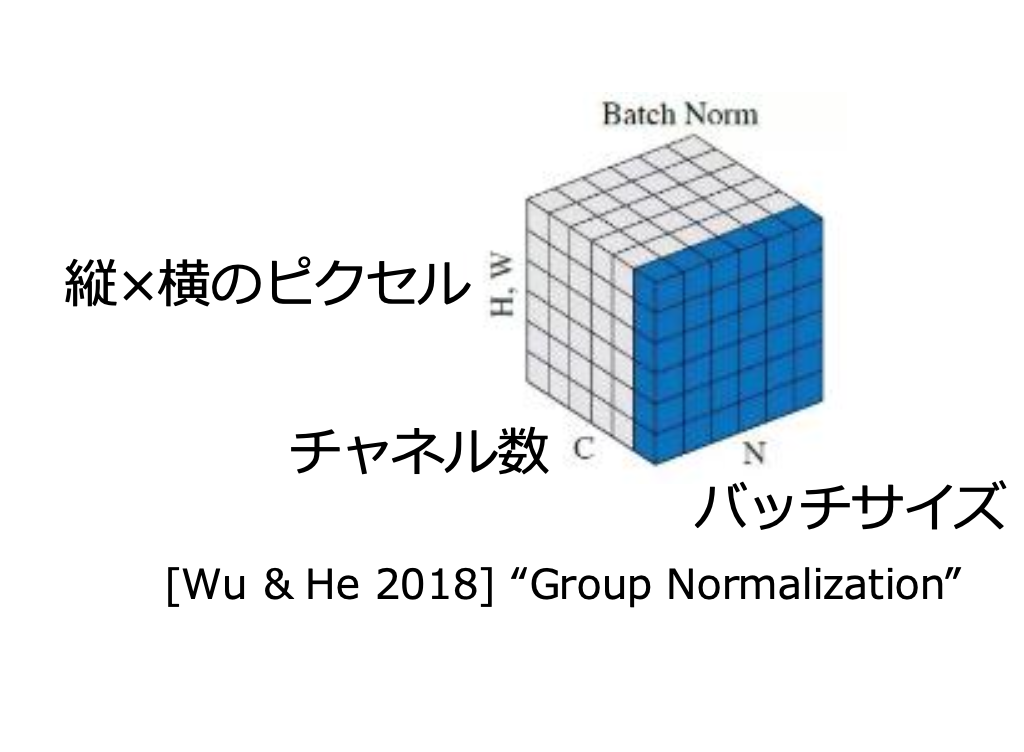
\includegraphics[width=0.6\textwidth]{Batch正規化.png}
    \caption*{各バッチ・チャンネルごとに正規化するイメージ}
  \end{figure}
  \vspace{-0.5em}
  推論時には訓練データの移動平均 $\mu_j,\sigma_j^2$ を使う  
\end{frame}

% Slide 5: Layer Normalization
\begin{frame}{3.6.4 レイヤー正規化 (Layer Normalization)}
  \begin{itemize}
    \item 各サンプルごとに,同じ層の全ユニット出力をまとめて正規化
      \[
        \mu = \frac{1}{J}\sum_{j=1}^J u_j,\quad
        \sigma^2 = \frac{1}{J}\sum_{j=1}^J (u_j - \mu)^2
      \]
    \item 正規化とアフィン変換
      \[
        \hat u_j
         = \frac{u_j - \mu}{\sqrt{\sigma^2 + \varepsilon}},\quad
        y_j = \gamma_j\,\hat u_j + \beta_j
      \tag{3.17}
      \]
    \item バッチに依存しないため,RNN のような繰り返し層にも適用可能
    \item 推論時も同一の計算を行うため,学習・推論で統計量のずれなし
  \end{itemize}
\end{frame}

\begin{frame}{レイヤー正規化 (Layer Normalization)}
  \[
    \mu = \frac1H\sum_{k=1}^H a_k, \quad
    \sigma^2 = \frac1H\sum_{k=1}^H (a_k-\mu)^2
  \]
  \[
    \hat a_k
      = \frac{a_k-\mu}{\sqrt{\sigma^2+\varepsilon}}, \quad
    y_k
      = \gamma_k\,\hat a_k + \beta_k
  \]
  \vspace{0.8em}
  \begin{figure}
    \centering
    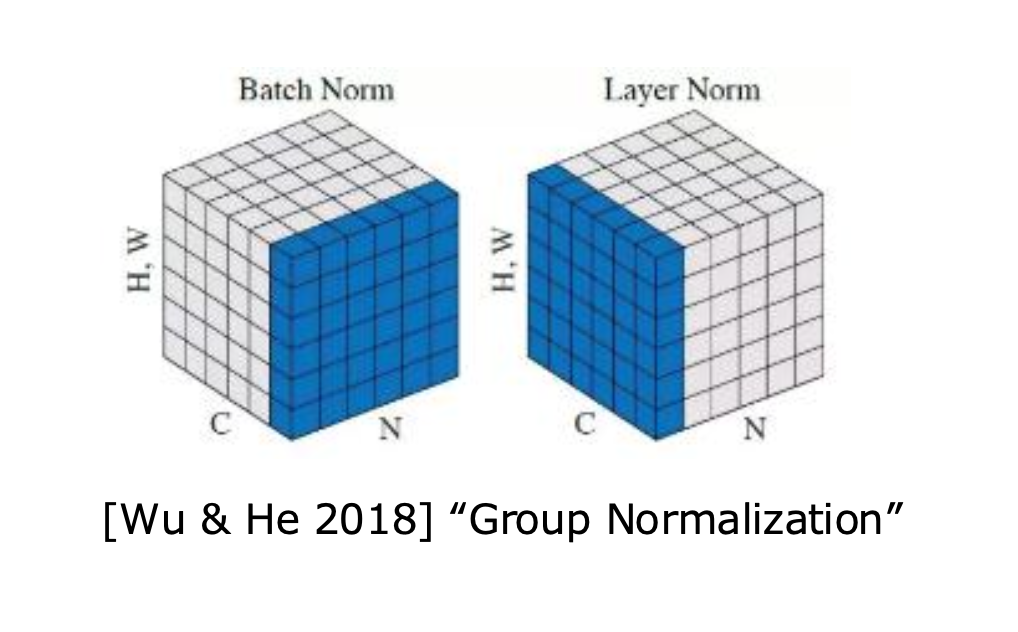
\includegraphics[width=0.6\textwidth]{Layer正規化.png}
    \caption*{レイヤー方向(チャンネル全体)で正規化するイメージ}
  \end{figure}
  \vspace{-0.5em}
  バッチサイズに依存せず,RNN や Transformer でも安定  
\end{frame}

\begin{frame}{インスタンス正規化 (Instance Normalization)}
  \begin{itemize}
    \item 各サンプル・各チャンネル単位で平均・分散を計算
    \item 小バッチサイズでも安定  
    \item 画像のスタイル変換(コントラスト正規化)に有効
  \end{itemize}
  \[
    \mu_{n,c} = \frac1{HW}\sum_{h=1}^H\sum_{w=1}^W x_{n,c,h,w}, \quad
    \sigma_{n,c}^2 = \frac1{HW}\sum_{h,w}(x_{n,c,h,w}-\mu_{n,c})^2
  \]
  \[
    \hat x_{n,c,h,w}
      = \frac{x_{n,c,h,w}-\mu_{n,c}}{\sqrt{\sigma_{n,c}^2+\varepsilon}}
  \]
  \vspace{0.8em}
  \begin{figure}
    \centering
    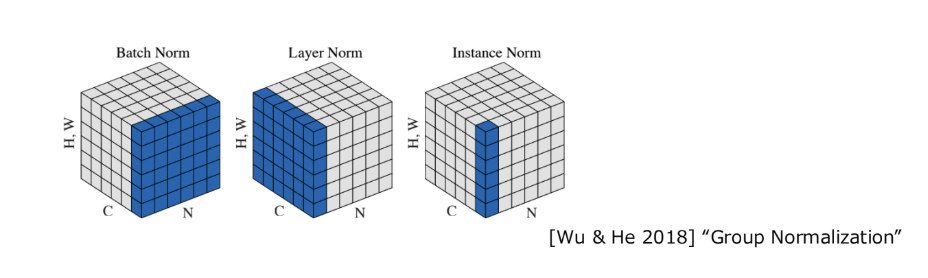
\includegraphics[width=0.6\textwidth]{Standalization.png}
    \caption*{各インスタンス・チャンネルごとに正規化するイメージ}
  \end{figure}
\end{frame}

% Slide 6: BatchNorm の欠点
\begin{frame}{3.6.5 バッチ正規化の欠点}
  \begin{itemize}
    \item 学習時と推論時で用いる統計量 $\mu_j,\;\sigma_j^2$ が異なる
    \item この統計量のずれが,ネットワークの出力に揺らぎを生じさせる
    \item 例:画像分類で入力画像サイズが学習時/推論時で異なるだけで性能低下が報告されている    \item そのため,BNを使わないネットワーク構造や学習法も提案されている
  \end{itemize}
\end{frame}

% Slide 7: Weight Normalization & Regularization
\begin{frame}{3.6.6 重みの正規化と正則化}
  \begin{itemize}
    \item 活性化関数を無視すると,層出力は
      \[
        y = w \, x
      \]
    \item 入力 $x$ が正規化済みなら,重みを正規化しても同様の効果が期待できる
      \[
        \mathbf{w} \;\longleftarrow\; \frac{\mathbf{w}}{\|\mathbf{w}\| + \varepsilon}
      \]
    \item この発想を用いた手法が「Weight Normalization」\cite{77,78,79}
    \item また,BN層でも L2 正則化(Weight Decay)
      \[
        L_{\rm reg} = \lambda \|\mathbf{w}\|^2
      \]
      は更新ダイナミクスを滑らかにし,有効性が認められている\cite{49}
  \end{itemize}
\end{frame}

\section{3.7}

\begin{frame}{層ごとの事前学習によるパラメータ初期化}
  \begin{itemize}
    \item \textbf{事前学習}  
      単純なタスクで単純なモデルを訓練し,得られたパラメータを次層の初期値とする戦略
    \item \textbf{貪欲教師あり事前学習}(Bengio \textit{et al.}, 2007)
      \begin{enumerate}
        \item 隠れ層1層のみを持つネットワークを教師ありで事前学習  
        \item その出力を固定し,次の層を1層だけ追加して再度教師あり事前学習  
        \item 必要な深さだけ繰り返し,良好な初期パラメータを得る
      \end{enumerate}
    \item 最近では層ごとの初期化の代わりに,特定の分布からのサンプリングで初期化
する方法が取られている
    \end{itemize}
\end{frame}

\begin{frame}{パラメータの初期化}
  \begin{itemize}
    \item \textbf{例1:一定幅の一様分布 (Uniform)}
      \[
        w_{p,q}^l \sim \mathrm{Uniform}(-0.05,\,0.05)
      \]
    \item \textbf{例2:平均0,標準偏差0.05のガウス分布}
      \[
        w_{p,q}^l \sim \mathcal{N}\bigl(0,\;0.05^2\bigr)
      \]
  \end{itemize}
\end{frame}

% ─────────────────────────────────────────────────────────────
% 勾配消失問題スライド
% ─────────────────────────────────────────────────────────────
\begin{frame}{ランダム初期化の問題:勾配消失}
  \begin{itemize}
    \item 活性化関数の勾配が小さい領域にパラメータが入ると  
          \(\nabla\) が伝達されず,学習が進まない
    \item シグモイド/Tanh の場合,入力が大きくなると  
          勾配(\(f'(u)\))がほぼ0に  
    \item ネットワークが深くなるほど顕著(多重に掛け合わされるため)
  \end{itemize}
\end{frame}


\begin{frame}{3.7 重みの初期化}
  \begin{itemize}
    \item 重みは学習開始時に初期化を行う
    \item 層ごとに確率分布 \(p(w)\) を定め,
      そこからランダム抽出して重み \(w_{ji}\) に設定
      \[
        w_{ji}\sim p(w)
      \]
    \item 一般的な選択例:
      \(\mathcal{N}(0,\sigma^2)\) あるいは
      \(U(-a,a)\)
    \item バイアスの初期値は通常 \(0\)
  \end{itemize}
\end{frame}

% Slide 2: 初期化の目的と前提
\begin{frame}{初期化における要請}
  \begin{itemize}
    \item 連続する層間で,層出力の大きさ(分散)が
      なるべく等しくなることが望ましい
    \item 順伝播・逆伝播の計算安定化に寄与
    \item 活性化関数に「スイートスポット」を持つ場合もあり
      (例:ロジスティック関数)
  \end{itemize}
\end{frame}

% Slide 3: 順伝播時の分散解析
\begin{frame}{順伝播時の分散解析}
  \[
    u'_j = \sum_{i=1}^M w_{ji}\,z_i,\quad
    z'_j = f(u'_j)
  \]
  \begin{align}
    V(u'_j)
      &= \sum_{i=1}^M V(w_{ji}z_i)
       = M\,V(w_{ji})\,E[z_i^2]
      \tag{3.18}\\
    % 活性化関数が原点対称で$f'(0)\approx1$のとき
    V(z'_j)
      &= M\,V(w_{ji})\,V(z_i)
      \tag{3.19}
  \end{align}
  \begin{block}{分散を保つ条件}
    \(V(z'_j)=V(z_i)\) とするには
    \[
      V(w_{ji}) = \frac{1}{M}
    \]
  \end{block}
\end{frame}

% Slide 4: Xavier(Glorot)初期化
\begin{frame}{Xavier(Glorot)初期化}
  \begin{itemize}
    \item 順伝播/逆伝播の両方を考慮し,
      ファンイン \(M\) とファンアウト \(M'\) の平均をとる
    \[
      V(w_{ji}) = \frac{2}{M + M'}
    \]
    \item 正規分布の場合:
      \(\displaystyle
        w_{ji}\sim\mathcal{N}\bigl(0,\sigma^2\bigr),\ 
        \sigma=\sqrt{\tfrac{2}{M+M'}}
      \)
    \item 一様分布の場合:
      \(\displaystyle
        w_{ji}\sim U(-a,a),\ 
        a=\sqrt{\tfrac{6}{M+M'}}
      \)
     \item \textbf{一様分布の分散導出}
      一様分布 \(U(-a,a)\) の分散は
      \(\displaystyle V=\frac{(2a)^2}{12}=\frac{a^2}{3}\) である。
      これを \(2/(n_{\rm in}+n_{\rm out})\) に合わせると
      \[
        \frac{a^2}{3} = \frac{2}{n_{\rm in}+n_{\rm out}}
        \;\Longrightarrow\;
        a = \sqrt{\frac{6}{n_{\rm in}+n_{\rm out}}}
      \] 
      と導出できる
    \item 通称:Xavier法/Glorot法
  \end{itemize}
  
\end{frame}
\begin{frame}{Xavier Initialization (Glorot 法)}
  \begin{itemize}
    \item 入力サイズ $n_{\rm in}$,出力サイズ $n_{\rm out}$ に応じた分散で初期化
    \[
      w_{p,q}^l \sim \mathcal{N}\Bigl(0,\frac{2}{n_{\rm in}+n_{\rm out}}\Bigr)
      \quad\text{または}\quad
      w_{p,q}^l \sim \mathrm{Uniform}\Bigl(-\frac{\sqrt{6}}{\sqrt{n_{\rm in}+n_{\rm out}}},\;\frac{\sqrt{6}}{\sqrt{n_{\rm in}+n_{\rm out}}}\Bigr)
    \]
    \item 動機:活性化関数が Sigmoid / Tanh の場合,順伝播・逆伝播で同じ分散を保つ  
      \[
        \mathrm{Var}(y) = \mathrm{Var}(x) = 1
        \;\Longrightarrow\;
        \mathrm{Var}(W)=\frac{2}{n_{\rm in}+n_{\rm out}}
      \]
  \end{itemize}
  \begin{figure}
    \centering
    \includegraphics[height=3cm]{tanh-sigmoid.png}
    \caption*{Tanh (青) と Sigmoid (緑) の出力分布イメージ}
  \end{figure}
\end{frame}

% Slide 5: Kaiming(He)初期化 & まとめ
\begin{frame}{Kaiming(He)初期化とまとめ}
  \begin{itemize}
    \item ReLU などの非負出力関数では
      \(E[z_i^2]=\tfrac12\,V(u_i)\) を利用
    \[
      V(w_{ji}) = \frac{2}{M}
      ,\quad
      \sigma = \sqrt{\tfrac{2}{M}}
      ,\quad
      a = \sqrt{\tfrac{6}{M}}
    \]
    \item 通称:Kaiming法/He法
  \end{itemize}
  \vspace{1em}
  \begin{table}
    \centering
    \begin{tabular}{lccc}
      \toprule
      メソッド & 分散条件 \(V(w)\) & \(\sigma\) & \(a\) \\
      \midrule
      Xavier (Glorot) & \(2/(M+M')\) 
        & \(\sqrt{2/(M+M')}\) & \(\sqrt{6/(M+M')}\) \\
      He (ReLU用)    & \(2/M\) 
        & \(\sqrt{2/M}\)      & \(\sqrt{6/M}\)      \\
      \bottomrule
    \end{tabular}
    \caption*{主な初期化手法の比較}
  \end{table}
\end{frame}

\begin{frame}{He Initialization (Kaiming 法)}
  \begin{itemize}
    \item ReLU の非負性を考慮し,分散を二倍に設定
    \[
\begin{aligned}
  \mathrm{Var}(W) &= \frac{2}{n_{\rm in}} \\[6pt]
  \Longrightarrow\quad
  w_{p,q}^l &\sim \mathcal{N}\!\Bigl(0,\tfrac{2}{n_{\rm in}}\Bigr), \\[6pt]
  w_{p,q}^l &\sim \mathrm{Uniform}\!\Bigl(-\tfrac{\sqrt{6}}{\sqrt{n_{\rm in}}},\,\tfrac{\sqrt{6}}{\sqrt{n_{\rm in}}}\Bigr)
\end{aligned}
\]

    \item 動機:ReLU の出力は半分が 0,残り半分で『1』近傍の勾配が伝播  
  \end{itemize}
  \begin{figure}
    \centering
    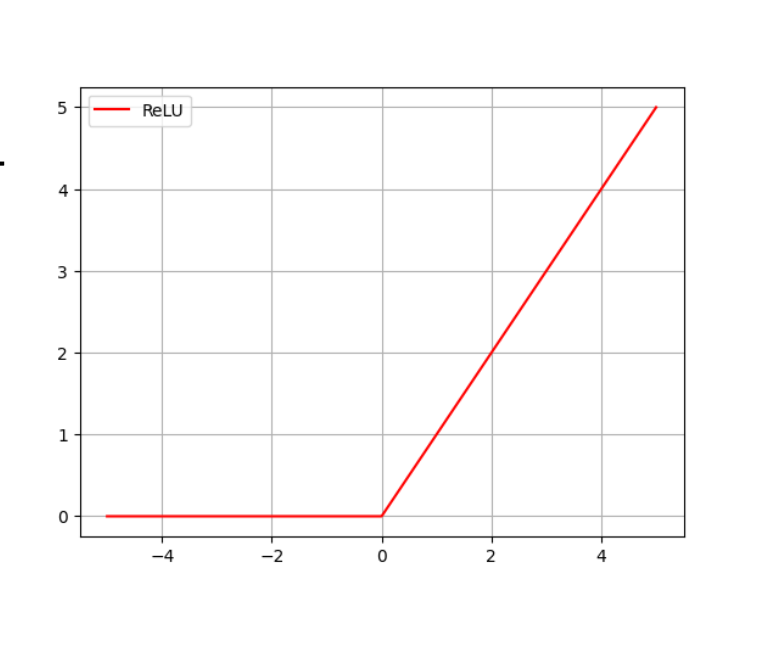
\includegraphics[height=3cm]{ReLU.png}
    \caption*{ReLU の出力イメージと勾配領域}
  \end{figure}
\end{frame}

\begin{frame}{初期化まとめ}
  \begin{itemize}
    \item 初期化方法により勾配が爆発/消失するリスクを抑制  
      活性化関数の非線形部に入りにくくするのが目的
    \item Bengio \textit{et al.} の事前学習(2007)は多層化の初期解を提供
    \item 近年は分布に基づく Xavier / He 法が主流  
      \begin{itemize}
        \item Sigmoid, Tanh:Xavier
        \item ReLU:He
      \end{itemize}
  \end{itemize}
\end{frame}

\section{3.8}
% ─────────────────────────────────────────────────────────────
% スライド1: カリキュラム学習
% ─────────────────────────────────────────────────────────────
\begin{frame}{カリキュラム学習の概要}
  \begin{itemize}
    \item ミニバッチの無差別サンプリングでは学習進度に応じた順序付けができない
    \item \textbf{カリキュラム学習 (Curriculum Learning)}
      \begin{itemize}
        \item 学習を易しいタスクから始め,徐々に難しいタスクへ移行
        \item 人間の学習プロセスを模倣し,効率的にパラメータ探索を促進
      \end{itemize}
    \item ただし,普遍的に有効と証明された手法は未だ存在しない
  \end{itemize}
\end{frame}

% ─────────────────────────────────────────────────────────────
% スライド2: 非凸損失関数と鞍点
% ─────────────────────────────────────────────────────────────
\begin{frame}{非凸損失関数と鞍点の問題}
  \begin{itemize}
    \item 深層ネットワークの損失関数は非凸で,多数の鞍点 (Saddle) を含む
    \item 鞍点では勾配が小さく,学習が停滞しやすい
    \item 実質的には「良い極小解 (Deep Minima)」を見つけられれば十分
  \end{itemize}
\end{frame}

\end{document}
